% !TeX root = RJwrapper.tex
\title{The R Package clustGLMM - Clustering Longitudinal Data of a Mixed Type}


\author{by Jan Vávra, Bettina Grün, Gertraud Malsiner-Walli, and Arnošt Komárek}

\maketitle

\abstract{%
An abstract of less than 150 words.
}

\section{Introduction}\label{introduction}

Our paper (Vávra et al. 2024). Our package \pkg{clustGLMM}.

We compare to \CRANpkg{lcmm} (Proust-Lima, Philipps, and Liquet 2017), \CRANpkg{mixAK}, \CRANpkg{flexmix}, \CRANpkg{MCMCglmm}. We take an inspiration from \CRANpkg{brms}.

\section{Background}\label{background}

Briefly explain the model, the use of model-based clustering and sparse finite mixtures and MCMC algorithm.

\subsection{Model}\label{model}

different distribution families

joint modelling of random effects

\subsection{Priors}\label{priors}

list of the used prior distributions + link with the parameters of \texttt{clustGLMM} function?

\subsection{Sparse finite mixtures}\label{sparse-finite-mixtures}

\texttt{Gplus} definition and prior for weights

\section{Implementation}\label{implementation}

\subsection{Scaling the numerical outcomes and regressors}\label{scaling-the-numerical-outcomes-and-regressors}

explain how the input data are scaled and how does it reference to model parameters

\subsection{MCMC estimation}\label{mcmc-estimation}

Gibbs + Metropolis-within-Gibbs steps

\subsection{clustering probabilities and deviance ?}\label{clustering-probabilities-and-deviance}

integral approximation

\section{Application}\label{application}

code+outputs

\subsection{Simulated students dataset}\label{simulated-students-dataset}

exemplary use of \pkg{clustGLMM} - step by step explanation and command introduction

\begin{verbatim}
#>    i  j g      age    income ntrips satisfaction     b_num      b_poi
#> 1  1  1 3 18.42013  95.01285      3            0 3.0835793 -0.3504447
#> 2  1  2 3 20.75503 103.02934      0            0 3.0835793 -0.3504447
#> 3  1  3 3 21.42530 108.03323      0            1 3.0835793 -0.3504447
#> 4  1  4 3 25.16883 127.68021      0            2 3.0835793 -0.3504447
#> 5  1  5 3 26.59334 152.50394      1            0 3.0835793 -0.3504447
#> 6  1  6 3 29.77266 160.85054      3            0 3.0835793 -0.3504447
#> 7  1  7 3 30.20771 167.06109      1            1 3.0835793 -0.3504447
#> 8  1  8 3 33.21026 160.19557      2            0 3.0835793 -0.3504447
#> 9  1  9 3 35.98933 169.31047      2            2 3.0835793 -0.3504447
#> 10 1 10 3 37.64983 174.34435      0            2 3.0835793 -0.3504447
#> 11 1 11 3 39.63856 185.52352      1            0 3.0835793 -0.3504447
#> 12 2  1 1 18.89800  96.27975      2            0 0.4688803 -0.3546576
#> 13 2  2 1 21.98552 109.00878      0            0 0.4688803 -0.3546576
#> 14 2  3 1 23.94263 118.72608      0            1 0.4688803 -0.3546576
#> 15 2  4 1 28.01344 110.67371      3            1 0.4688803 -0.3546576
#>         b_ord
#> 1   0.1348468
#> 2   0.1348468
#> 3   0.1348468
#> 4   0.1348468
#> 5   0.1348468
#> 6   0.1348468
#> 7   0.1348468
#> 8   0.1348468
#> 9   0.1348468
#> 10  0.1348468
#> 11  0.1348468
#> 12 -0.5328982
#> 13 -0.5328982
#> 14 -0.5328982
#> 15 -0.5328982
\end{verbatim}

\begin{verbatim}
#>        i               j                g              age       
#>  Min.   :  1.0   Min.   : 1.000   Min.   :1.000   Min.   :18.00  
#>  1st Qu.:125.8   1st Qu.: 3.000   1st Qu.:1.000   1st Qu.:22.97  
#>  Median :250.0   Median : 5.000   Median :2.000   Median :28.95  
#>  Mean   :250.2   Mean   : 5.072   Mean   :1.882   Mean   :29.01  
#>  3rd Qu.:375.2   3rd Qu.: 7.000   3rd Qu.:3.000   3rd Qu.:35.06  
#>  Max.   :500.0   Max.   :14.000   Max.   :3.000   Max.   :40.00  
#>      income           ntrips       satisfaction     b_num        
#>  Min.   : 48.71   Min.   : 0.000   0:1319       Min.   :-9.7207  
#>  1st Qu.:112.32   1st Qu.: 1.000   1:1837       1st Qu.:-1.7550  
#>  Median :135.28   Median : 2.000   2:1356       Median : 0.1311  
#>  Mean   :134.36   Mean   : 3.239                Mean   : 0.1457  
#>  3rd Qu.:155.39   3rd Qu.: 4.000                3rd Qu.: 2.2994  
#>  Max.   :213.66   Max.   :32.000                Max.   : 8.4850  
#>      b_poi              b_ord          
#>  Min.   :-1.41302   Min.   :-1.437139  
#>  1st Qu.:-0.38789   1st Qu.:-0.358931  
#>  Median :-0.02384   Median : 0.008360  
#>  Mean   :-0.01930   Mean   : 0.002852  
#>  3rd Qu.: 0.34478   3rd Qu.: 0.357413  
#>  Max.   : 1.71043   Max.   : 1.423791
\end{verbatim}

\begin{verbatim}
#> $`1`
#>    Min. 1st Qu.  Median    Mean 3rd Qu.    Max. 
#>   77.23  112.79  128.98  126.99  141.68  176.05 
#> 
#> $`2`
#>    Min. 1st Qu.  Median    Mean 3rd Qu.    Max. 
#>   61.79  111.55  143.41  137.56  164.23  199.46 
#> 
#> $`3`
#>    Min. 1st Qu.  Median    Mean 3rd Qu.    Max. 
#>   48.71  112.08  147.42  141.37  169.35  213.66
\end{verbatim}

\begin{verbatim}
#> $`1`
#>    Min. 1st Qu.  Median    Mean 3rd Qu.    Max. 
#>   0.000   1.000   3.000   3.411   5.000  19.000 
#> 
#> $`2`
#>    Min. 1st Qu.  Median    Mean 3rd Qu.    Max. 
#>   0.000   1.000   3.000   3.859   5.000  32.000 
#> 
#> $`3`
#>    Min. 1st Qu.  Median    Mean 3rd Qu.    Max. 
#>   0.000   1.000   2.000   2.344   3.000  23.000
\end{verbatim}

\begin{verbatim}
#> $`1`
#>   0   1   2 
#> 503 808 525 
#> 
#> $`2`
#>   0   1   2 
#> 251 508 613 
#> 
#> $`3`
#>   0   1   2 
#> 565 521 218
\end{verbatim}

\begin{figure}
\centering
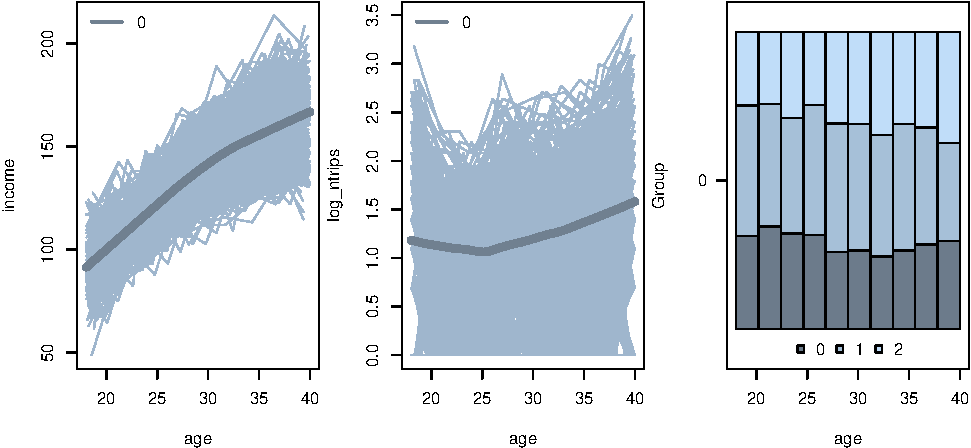
\includegraphics{figure-latex/plot-students-blind-1.pdf}
\caption{\label{fig:plot-students-blind}Outcomes vs age without knowledge of the grouping.}
\end{figure}

\begin{figure}
\centering
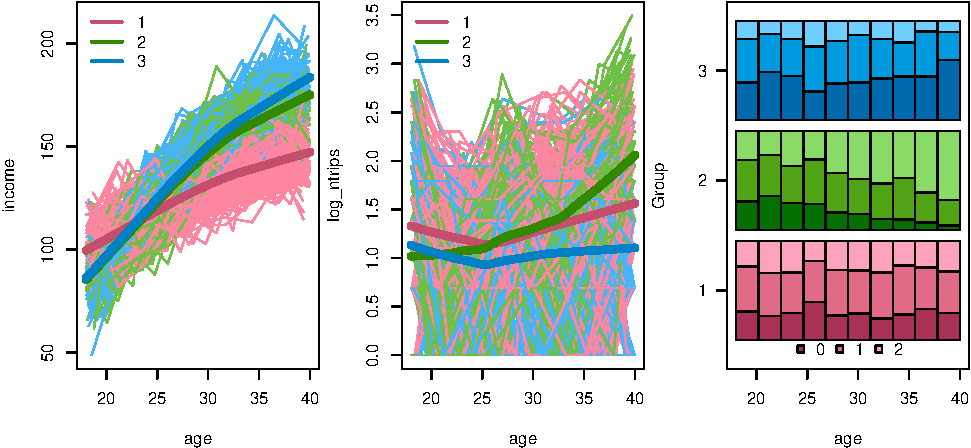
\includegraphics{figure-latex/plot-students-grouped-1.pdf}
\caption{\label{fig:plot-students-grouped}Outcomes vs age with the true grouping.}
\end{figure}

\subsubsection{\texorpdfstring{\texttt{clustGLMM}}{clustGLMM}}\label{clustglmm}

how to prepare the call of \texttt{clustGLMM}

\subsubsection{Summaries and plots}\label{summaries-and-plots}

what plots and summaries can be obtained from \texttt{clustglmm} class object

\subsubsection{\texorpdfstring{\texttt{post\_processing}}{post\_processing}}\label{post_processing}

explain how post processing works and how the user can work with the post-processed family

\subsubsection{\texorpdfstring{\texttt{clustering\_probabilities\_and\_deviance}}{clustering\_probabilities\_and\_deviance}}\label{clustering_probabilities_and_deviance}

approximation of the clustering probabilities and deviance

\subsection{\texorpdfstring{Analysis of \texttt{paquid} dataset from \pkg{lcmm}}{Analysis of paquid dataset from }}\label{analysis-of-paquid-dataset-from}

direct analysis analogical to the one performed in \pkg{lcmm} + what are our advantages

\section{Summary}\label{summary}

\pkg{clustGLMM} is very flexible and provides more than existing packages.

Future outlooks:

\begin{itemize}
\tightlist
\item
  more families,
\item
  semi-supervised approach,
\item
  higher flexibility with \texttt{prec\_num} and \texttt{c\_ord} parameters.
\end{itemize}

\section*{References}\label{references}
\addcontentsline{toc}{section}{References}

\phantomsection\label{refs}
\begin{CSLReferences}{1}{0}
\bibitem[\citeproctext]{ref-Proust-Lima-etal2017}
Proust-Lima, Cécile, Viviane Philipps, and Benoit Liquet. 2017. {``Estimation of Extended Mixed Models Using Latent Classes and Latent Processes: The r Package Lcmm.''} \emph{Journal of Statistical Software} 78 (2): 1--56. \url{https://doi.org/10.18637/jss.v078.i02}.

\bibitem[\citeproctext]{ref-Vavra-etal2024}
Vávra, Jan, Arnošt Komárek, Bettina Grün, and Gertraud Malsiner-Walli. 2024. {``Clusterwise Multivariate Regression of Mixed-Type Panel Data.''} \emph{Statistics and Computing} 34 (46). \url{https://doi.org/10.1007/s11222-023-10304-5}.

\end{CSLReferences}


\address{%
Jan Vávra\\
Charles University\\%
Sokolovská 49/83\\ 186 75 Praha 8\\
Vienna University of Economics and Bussiness\\%
Welthandelsplatz 1\\ 1020 Wien\\
%
\url{https://www2.karlin.mff.cuni.cz/~vavraj/}\\%
\textit{ORCiD: \href{https://orcid.org/0000-0003-0068-5356}{0000-0003-0068-5356}}\\%
\href{mailto:vavraj@karlin.mff.cuni.cz}{\nolinkurl{vavraj@karlin.mff.cuni.cz}}%
}

\address{%
Bettina Grün\\
Vienna University of Economics and Bussiness\\%
Welthandelsplatz 1\\ 1020 Wien\\
%
\url{https://research.wu.ac.at/de/persons/bettina-gr\%C3\%BCn-7}\\%
\textit{ORCiD: \href{https://orcid.org/0000-0001-7265-4773}{0000-0001-7265-4773}}\\%
\href{mailto:bettina.gruen@wu.ac.at}{\nolinkurl{bettina.gruen@wu.ac.at}}%
}

\address{%
Gertraud Malsiner-Walli\\
Vienna University of Economics and Bussiness\\%
Welthandelsplatz 1\\ 1020 Wien\\
%
\url{https://research.wu.ac.at/de/persons/gertraud-malsiner-walli-3}\\%
\textit{ORCiD: \href{https://orcid.org/0000-0002-1213-4749}{0000-0002-1213-4749}}\\%
\href{mailto:gertraud.malsiner-walli@wu.ac.at}{\nolinkurl{gertraud.malsiner-walli@wu.ac.at}}%
}

\address{%
Arnošt Komárek\\
Charles University\\%
Sokolovská 49/83\\ 186 75 Praha 8\\
%
\url{https://msekce.karlin.mff.cuni.cz/~komarek/}\\%
\textit{ORCiD: \href{https://orcid.org/0000-0001-8778-3762}{0000-0001-8778-3762}}\\%
\href{mailto:arnost.komarek@mff.cuni.cz}{\nolinkurl{arnost.komarek@mff.cuni.cz}}%
}
